\documentclass{../../note}

\usepackage{amsthm}
\usepackage{pgfplots}
\pgfplotsset{compat=1.18}
\usepackage{xcolor}
\usepackage{tikz}
\usetikzlibrary{shapes,arrows,positioning,fit,calc,matrix,decorations.pathreplacing}
\usepackage{algorithm}
\usepackage{algpseudocode}
\usepackage{listings}
\usepackage{booktabs}
\usepackage{array}
\usepackage{enumitem}

\lstset{
  basicstyle=\ttfamily\small,
  keywordstyle=\color{blue},
  commentstyle=\color{green!60!black},
  stringstyle=\color{purple},
  numbers=left,
  numberstyle=\tiny,
  numbersep=5pt,
  breaklines=true,
  frame=single,
}

\title{HUFE 数据结构模拟试卷 A}
\author{isomo}
\setlength{\parindent}{0em}

\begin{document}

\fontsize{12pt}{14.4pt}\selectfont
\maketitle

本卷依据最新考纲与课程时间安排整理，覆盖线性表、栈和队列、树与二叉树、图、查找与排序等高频考点。

\section*{一、填空题（10空，每空2分，共20分）}

\begin{enumerate}[itemsep=0.8em]
\item 一个算法的效率通常从\underline{\hspace{2cm}}复杂度和\underline{\hspace{2cm}}复杂度两个方面进行分析。
\item 向一个长度为 $n$ 的顺序表中删除第 $i$ 个元素（$1 \le i \le n$）时，需要向前移动\underline{\hspace{2cm}}个元素。
\item 栈具有\underline{\hspace{2cm}}的特性，队列具有\underline{\hspace{2cm}}的特性。
\item 在树形结构中，根结点没有\underline{\hspace{2cm}}结点；除根结点外，其余每个结点有且只有一个\underline{\hspace{2cm}}结点。
\item 已知一棵二叉树的先序序列和\underline{\hspace{2cm}}序列，一般不能唯一确定该二叉树。
\item 高度为 $h$ 的完全二叉树最多有\underline{\hspace{2cm}}个结点。
\item 图的深度优先遍历在实现思想上类似于二叉树的\underline{\hspace{2cm}}遍历。
\item 二叉排序树中，对其进行\underline{\hspace{2cm}}遍历可以得到一个递增序列。
\item 折半查找要求查找表既是\underline{\hspace{2cm}}存储结构，又按关键字有序。
\item 直接插入排序在最好情况下的时间复杂度为\underline{\hspace{2cm}}。
\end{enumerate}

\section*{二、单项选择题（10题，每题2分，共20分）}

\begin{enumerate}[itemsep=0.8em]
\item 计算机算法指的是（\hspace{0.8cm}）。

A．计算方法 \quad B．解决问题的有限运算序列 \quad C．排序方法 \quad D．调度方法

\item 线性表采用链式存储结构时，存储单元地址（\hspace{0.8cm}）。

A．必须连续 \quad B．部分必须连续 \quad C．一定不连续 \quad D．可以连续也可以不连续

\item 若一个栈的入栈序列为 $1,2,3,4,5$，则下列不可能的出栈序列是（\hspace{0.8cm}）。

A．5,4,3,2,1 \quad B．2,1,4,3,5 \quad C．3,1,2,5,4 \quad D．1,2,3,4,5

\item 循环队列中，若队列大小为 $m$，则判定队满的条件是（\hspace{0.8cm}）。

A．$front=rear$ \quad B．$(rear+1)\bmod m=front$ \quad C．$rear=m-1$ \quad D．$front=-1$

\item 哈夫曼树中度为 1 的结点个数是（\hspace{0.8cm}）。

A．0 \quad B．1 \quad C．2 \quad D．不确定

\item 下列关于图的叙述中，正确的是（\hspace{0.8cm}）。

A．有向图的邻接矩阵一定关于主对角线对称
\quad B．无向图中每条边对应两个方向
\quad C．图的遍历只能采用递归实现
\quad D．邻接表适合表示稀疏图

\item 对长度为 $n$ 的有序顺序表进行折半查找，在最坏情况下需要比较的关键字次数为（\hspace{0.8cm}）。

A．$O(1)$ \quad B．$O(\log n)$ \quad C．$O(n)$ \quad D．$O(n\log n)$

\item 在下列排序方法中，稳定且平均时间复杂度为 $O(n\log n)$ 的是（\hspace{0.8cm}）。

A．快速排序 \quad B．简单选择排序 \quad C．归并排序 \quad D．堆排序

\item 若一棵非空二叉树的叶子结点数为 $n_0$，度为 2 的结点数为 $n_2$，则必有（\hspace{0.8cm}）。

A．$n_0=n_2$ \quad B．$n_0=n_2+1$ \quad C．$n_0=2n_2$ \quad D．$n_0=n_2-1$

\item 在哈希表中处理冲突的方法不包括（\hspace{0.8cm}）。

A．开放定址法 \quad B．链地址法 \quad C．折半查找法 \quad D．再散列法
\end{enumerate}

\section*{三、判断题（10题，每题1分，共10分）}

\begin{enumerate}[itemsep=0.6em]
\item 线性表的顺序存储结构一定优于链式存储结构。 （\hspace{0.8cm}）
\item 栈和队列都是操作受限的线性表。 （\hspace{0.8cm}）
\item 哈夫曼树中不存在度为 1 的结点。 （\hspace{0.8cm}）
\item 由一棵二叉树的先序序列和后序序列可以唯一确定该二叉树。 （\hspace{0.8cm}）
\item 一个无向图的邻接矩阵是对称矩阵。 （\hspace{0.8cm}）
\item 二叉排序树的中序遍历结果一定是有序的。 （\hspace{0.8cm}）
\item 直接插入排序和冒泡排序都属于稳定排序。 （\hspace{0.8cm}）
\item 若某排序算法不稳定，则它没有实际应用价值。 （\hspace{0.8cm}）
\item 对于频繁插入和删除的线性表，链式存储通常比顺序存储更合适。 （\hspace{0.8cm}）
\item 广度优先遍历图时通常需要借助队列。 （\hspace{0.8cm}）
\end{enumerate}

\section*{四、简答题（4题，每题5分，共20分）}

\begin{enumerate}[itemsep=1em]
\item 简述顺序表与单链表在存储方式、插入删除效率、随机访问能力方面的主要区别。
\item 设某栈的输入序列为 A，B，C，D，E。判断下列序列能否作为其出栈序列，并说明理由：
\begin{enumerate}[label=(\arabic*)]
\item B，A，E，D，C
\item C，E，A，D，B
\end{enumerate}
\item 什么是二叉排序树？删除二叉排序树中某个结点时通常需要分哪三种情况处理？
\item 比较直接插入排序、冒泡排序和简单选择排序的基本思想，并指出其中哪些算法是稳定的。
\end{enumerate}

\section*{五、综合应用题（3题，每题10分，共30分）}

\begin{enumerate}[itemsep=1.2em]
\item 已知某二叉树的先序序列为 \texttt{ABDECFG}，中序序列为 \texttt{DBEAFCG}。
\begin{enumerate}[label=(\arabic*)]
\item 画出该二叉树；
\item 写出该二叉树的后序遍历序列；
\item 求该二叉树的叶子结点。
\end{enumerate}

\item 已知无向带权图 $G$ 如下图所示，请回答下列问题：
\begin{enumerate}[label=(\arabic*)]
\item 从顶点 A 出发写出一种深度优先遍历序列；
\item 从顶点 A 出发写出一种广度优先遍历序列；
\item 用 Prim 算法求该图的一棵最小生成树，并写出选边过程。
\end{enumerate}

\begin{center}
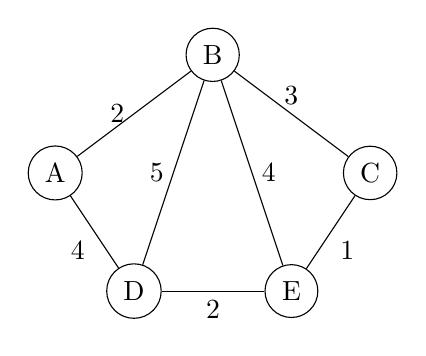
\begin{tikzpicture}[scale=1]
  \node[circle,draw] (A) at (0,1.5) {A};
  \node[circle,draw] (B) at (2,3) {B};
  \node[circle,draw] (C) at (4,1.5) {C};
  \node[circle,draw] (D) at (1,0) {D};
  \node[circle,draw] (E) at (3,0) {E};

  \draw (A) -- node[left] {2} (B);
  \draw (A) -- node[below left] {4} (D);
  \draw (B) -- node[above] {3} (C);
  \draw (B) -- node[left] {5} (D);
  \draw (B) -- node[right] {4} (E);
  \draw (C) -- node[below right] {1} (E);
  \draw (D) -- node[below] {2} (E);
\end{tikzpicture}
\end{center}

\item 已知关键字序列为 $\{27,18,32,18,41,22,44,59\}$。
\begin{enumerate}[label=(\arabic*)]
\item 用直接插入排序对该序列进行升序排序，写出前两趟排序结果；
\item 若哈希函数为 $H(key)=key\bmod 7$，采用链地址法构造哈希表，给出每个地址上的关键字；
\item 说明折半查找为什么不能直接用于该原始序列。
\end{enumerate}
\end{enumerate}

\end{document}
